\lab{Applications}{Wavelet Denoising and Compression}{Denoising and Compression}

\objective{This lab presents the two-dimensional Discrete Wavelet Transform
as well as related applications in image denoising and compression.}

\section*{The two-dimensional Discrete Wavelet Transform}
In the previous lab, we explored wavelet analysis using the Haar wavelet and
the discrete wavelet transform. Our discussion focused on one-dimensional
discrete signals, but it is not difficult to extend the same ideas into the
realm of two-dimensional arrays. As you know, a digital image can be represented
as a matrix of pixel values (for simplicity we will consider grayscale images of
size $2^n \times 2^n$ in this lab). We can perform the wavelet decomposition of
an image in much that same way as with one-dimensional signals. We once again
calculate detail and approximation coefficients using an iterative filter
bank, but now we generate four arrays of coefficients at each iteration as opposed to
just two. In essence, we perform the one-dimensional wavelet transform first on each
row, and then on each column of the matrix. Given an input matrix of size $2^n \times
2^n$, after operating on the rows, we have two matrices of size $2^n \times 2^{n-1}$,
since each row has been downsampled by a factor of 2. Then for each of these two
intermediate matrices, operate on each column, yielding a total of four matrices of
size $2^{n-1} \times 2^{n-1}$. Recall the issues associated with the function
\li{sp.signal.fftconvolve} discussed in the previous lab. Figure \ref{fig:2dwt}
gives a graphical depiction of one iteration of the algorithm.

\begin{figure}[t]
    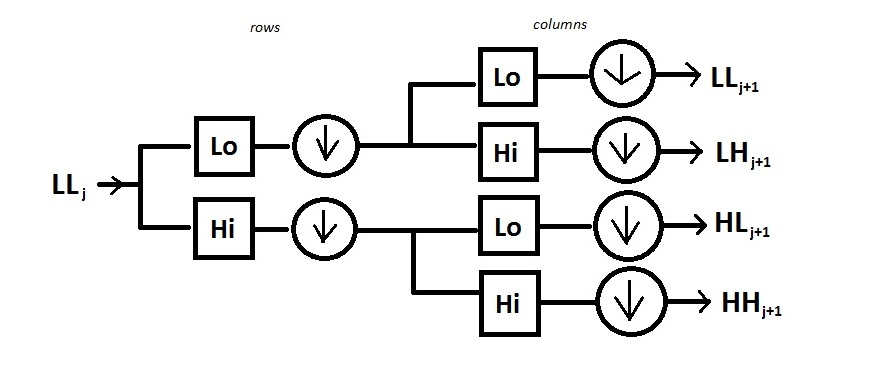
\includegraphics[width=0.8\textwidth]{2dwt.jpg}
    \caption{The 2-dimensional discrete wavelet transform.}
    \label{fig:2dwt}
\end{figure}


We initialize $LL_0$ to be the
original image matrix, and we terminate once the length of the rows or columns
is less than the length of the filters. We end up with a list of wavelet
coefficients, starting with the final approximation frame $LL_n$ followed by
collections of detail coefficients $(LH_n,HL_n,HH_n)$, $(LH_{n-1},HL_{n-1},HH_{n-1})$,
$\ldots$, $(LH_1,HL_1,HH_1)$. Note that at each iteration we operate first on the
rows (convolve with the filter, then downsample), and the we operate on the columns
of the resulting matrices (\emph{not} the original matrix). The size of the output
matrices have been reduced by a factor of two in both dimensions. As with the
one-dimensional algorithm, to reconstruct the image from the coefficients, we simply
reverse the process by upsampling, convolving, and adding (first the columns, then
the rows). Here is some sample code for one iteration of the transform and the inverse.

\begin{lstlisting}
def dwt2_pass(image,lo_d,hi_d):
	temp = sp.zeros([image.shape[0], image.shape[1]/2])
	LL = sp.zeros([image.shape[0]/2, image.shape[1]/2])
    LH = sp.zeros([image.shape[0]/2, image.shape[1]/2])    
	for i in xrange(image.shape[0]):
		temp[i] = sp.signal.fftconvolve(image[i], lo_d, mode='full')[1::2]    
	for i in xrange(image.shape[1]/2):    
		LL[:,i] = sp.signal.fftconvolve(temp[:,i],lo_d,mode='full')[1::2]    
        LH[:,i] = sp.signal.fftconvolve(temp[:,i],hi_d,mode='full')[1::2]  
	HL = sp.zeros([image.shape[0]/2, image.shape[1]/2])        
    HH = sp.zeros([image.shape[0]/2, image.shape[1]/2])        
	for i in xrange(image.shape[0]):        
		temp[i] = sp.signal.fftconvolve(image[i], hi_d, mode='full')[1::2]        
	for i in xrange(image.shape[1]/2):        
		HL[:,i] = sp.signal.fftconvolve(temp[:,i],lo_d,mode='full')[1::2]
        HH[:,i] = sp.signal.fftconvolve(temp[:,i],hi_d,mode='full')[1::2] 	return [LL,LH,HL,HH]

def idwt2_pass(coeffs, lo_r, hi_r):
	LL, LH, HL, HH = coeffs
    n = LL.shape[0]
	temp1 = sp.zeros([2*n,n])
	temp2 = sp.zeros([2*n,n])
	up1 = sp.zeros(2*n)
	up2 = sp.zeros(2*n) 
	for i in xrange(n):
		up1[1::2] = HH[:,i]
		up2[1::2] = HL[:,i]
		temp1[:,i] = fftconvolve(up1, hi_r)[1:] + fftconvolve(up2, lo_r)[1:]
		up1[1::2] = LH[:,i]
		up2[1::2] = LL[:,i]		
		temp2[:,i] = fftconvolve(up1, hi_r)[1:] + fftconvolve(up2, lo_r)[1:]
	result = sp.zeros([2*n,2*n])
	for i in xrange(2*n):
		up1[1::2] = temp1[i]
		up2[1::2] = temp2[i]
		result[i] = fftconvolve(up1, hi_r)[1:] + fftconvolve(up2, lo_r)[1:]
	return result
\end{lstlisting}

\begin{problem}
Build off of the sample code to fully implement the two-dimensional discrete 
wavelet transform as described above.
As in the last lab, the input to your decomposition function should consist of
three arrays: the input image, the low-pass filter, and the high-pass filter.
To increase the flexibility, also include an integer parameter that determines
the level of the decomposition, i.e. how many iterations to perform. Have the
default value of this parameter cause the function to compute the complete
decomposition.
You should return a list of the following form: $[LL_n,[LH_n,HL_n,HH_n],\ldots
,[LH_1,HL_1,HH_1]]$. The reconstruction function should take as input a list
of that same form, as well as the reconstruction low-pass and high-pass filters,
and should return the reconstructed image.
\end{problem}

These wavelet coefficients are very useful in a variety of image processing
tasks. They allow us to analyze and manipulate images in terms of both their
frequency and spatial properties, and at differing levels of resolution.
Furthermore, wavelet bases often have the remarkable ability to represent
images in a very \textit{sparse} manner -- that is, most of the image
information is captured by a small subset of the wavelet coefficients.
In the remainder of this lab, we will see how the discrete wavelet transform
plays a role in edge detection, noise removal, and compression.

\section*{Edge Detection}
It is often useful to identify the edges of objects and figures
represented in images. The edge information can be used to classify images
and group them with other similar images (this is part of a field called
\textit{computer vision}), to segment the image into component parts, to
sharpen blurry images, to filter out unnecessary details of the image,
and so forth. Of course, our human eyes are very adept at recognizing edges,
but enabling a computer to do the same is much more difficult. An edge can
be thought of as a discontinuity in the image or a region of high contrast
in either color or brightness. We can therefore leverage the high-frequency
detail coefficients of the wavelet transform to detect the edges. Once again
using the Haar Wavelet and its associated filters, execute the following
code:
\begin{lstlisting}
import numpy as np
from scipy.misc import imread
from matplotlib import pyplot as plt
from matplotlib import cm

# Get the standard Lenna image for processing
lenna = np.array(imread("Lenna.png",flatten=True),dtype=np.float32)

# Use your 2-dimensional DWT function to calculate one level of coefficients
coeffs = dwt2(lenna,lo_d,hi_d,1)

# Now visualize the original image together with the result
top = np.vstack([coeffs[0]/2.0,np.absolute(coeffs[1][0])])
bottom = np.vstack([np.absolute(coeffs[1][1]),np.absolute(coeffs[1][2])])
plt.imshow(np.hstack([lenna,np.hstack([top,bottom])),cmap=cm.Greys_r)
plt.show()
\end{lstlisting}

Note that the approximation coefficients are very close to the original
image, while the detail coefficients are much more sparse, and roughly
capture the edges in the image. In particular, the upper right coefficients
emphasize the vertical edges, the lower left coefficients emphasize the
horizontal edges, and the lower right coefficients emphasize the diagonal
edges.

\begin{problem}
Now zero out the approximation coefficients and use your inverse DWT
function to recreate the image. Plot its absolute value. This image is
a fairly good representation of the edges. If we add this to the original
image, we can increase the contrast at the edges (that is, make the dark
side darker, and the light side lighter). Do this, and plot the original
image side-by-side with the sharpened image. What do you notice? There
are many image-sharpening techniques, and those based on wavelets
are more sophisticated than what we have done here, but this gives the
basic idea.
\end{problem}

\section*{Noise Removal}
Noise in an image can be defined as unwanted visual artifacts that
obscure the true image. Images can acquire noise from a variety of
sources, including the camera, transmission, and image processing
algorithms. Noise can be completely random and incoherent (as in
Figure \ref{fig:incoherent}), or it can be coherent and display
visual patterns (Figure \ref{fig:coherent}). In this section, we will
focus on reducing a particular type of random noise in images, called
\textit{Gaussian white noise}.

\begin{figure}[t]
\minipage{0.49\textwidth}
    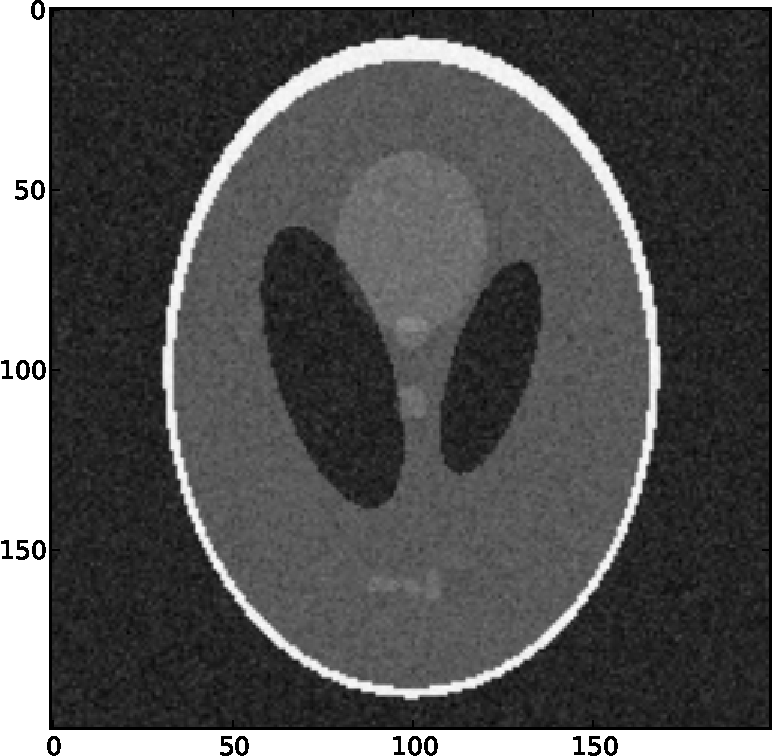
\includegraphics[width=\linewidth]{phantom_random.pdf}
    \caption{The Phantom image with incoherent noise}
    \label{fig:incoherent}
\endminipage\hfill
\minipage{0.49\textwidth}
    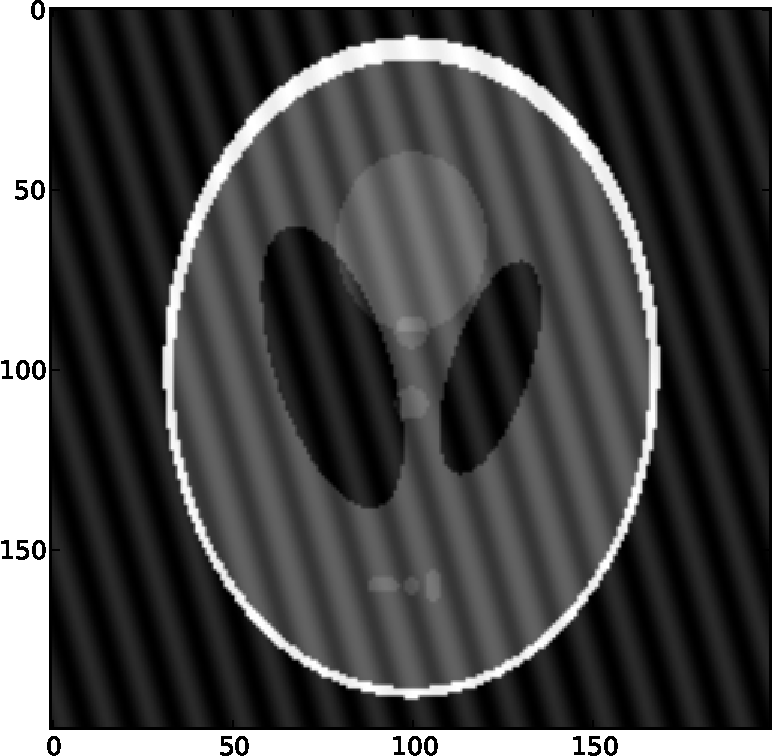
\includegraphics[width=\linewidth]{phantom_coherent.pdf}
    \caption{The Phantom image with coherent noise}
    \label{fig:coherent}
\endminipage
\end{figure}

An image that is distorted by Gaussian white noise is one in which
every pixel has been perturbed by a small amount, such that the
perturbations are normally distributed. We can easily add such noise
to an image using the \li{np.random.normal} function.

Given an image with Gaussian white noise, how do we go about reducing
the noise level? Our approach will be based on the idea of thresholding.
As discussed earlier, images are often sparse in the wavelet basis,
particularly in the high-frequency details. The Gaussian noise, however,
is very high frequency, and thus its wavelet transform will be
concentrated in high-frequency wavelet coefficients (of magnitude
roughly proportional to the variance of the noise). We can therefore
reduce the noise while preserving the true image by shrinking the
detail coefficients via hard or soft thresholding.

Given a positive threshold value $\tau$, hard thresholding sets
every wavelet coefficient whose magnitude is less than $\tau$ to
zero, while leaving the remaining coefficients untouched. Soft
thresholding also zeros out all coefficients of magnitude less than
$\tau$, but in addition maps every other coefficient $\beta$ to
$\beta - \tau$ if $\beta > 0$ or $\beta + \tau$ if $\beta < 0$.

Once the coefficients have been thresholded, we take the inverse
wavelet transform to recover the denoised image. The threshold
value is generally a function of the variance of the noise,
and in real situations, we do not know what this variance is. In fact,
noise variance estimation in images is a research area in its own
right, but this goes beyond the scope of this lab, and so we will
assume that we already have a decent estimate of the variance.

\begin{problem}
Write functions that implement the hard and soft thresholding
techniques. The inputs should be a list of wavelet coefficients
in standard form, as well as the threshold value. The output
should be the thresholded wavelet coefficients (also in
standard form). Remember that we only want to threshold the
detail coefficients, and not the approximation coefficients.
You should therefore leave the first entry of the input
coefficient list unchanged.
\end{problem}
\begin{problem}
Create a noisy version of the Lenna image by adding Gaussian
white noise of mean 0 and standard deviation $\sigma = 20$. Compute four
levels of the wavelet coefficients, and input these into your
thresholding functions (with $\tau = 3\sigma$ for the hard threshold,
and $\tau = 3\sigma/2$ for the soft threshold). Reconstruct the
two denoised images, and then plot these together alongside the
noisy image. What do you notice? How does lowering or raising the
threshold affect the reconstructed images?
\end{problem}

\section*{Image Compression}
We now turn to the problem of image compression. Explicitly saving
the value of every pixel in an image can be very costly in both
storage and transmission, and numerous image compression techniques
have been developed over the years to deal with this problem.
Transform methods have long played an important role in these
techniques; the popular JPEG image compression standard is based on
the discrete cosine transform. Starting from the early 1990's, much
research has gone into compression methods using the discrete wavelet
transform, and to great success. The JPEG2000 compression standard
and the FBI Fingerprint Image database, along with other systems,
take the wavelet approach.

The general framework for compression is fairly straightforward. First,
the image to be compressed undergoes some form of preprocessing (this
can include subtracting out its mean, tiling the image, or perhaps
nothing at all). Next, the wavelet coefficients are computed using some
specially constructed wavelet (JPEG2000 uses the either the
Cohen-Daubechies-Feauveau 9/7 or 5/3 wavelet) and then \textit{quantized},
 a process that we will explain shortly. The quantized coefficients are
 then grouped in a particular way and passed through an entropy encoder
 (such as Huffman coding, run length coding, or arithmetic coding). This
 coding step comes from the realm of information theory, and we will not
 worry about it in this lab. What you have left is a compact stream of bits
 that can then be saved or transmitted much more efficiently than the
 original image. All of the above steps are invertible, allowing us to
 reconstruct the image from the bitstream.

 The step in this process that we will focus on is quantization. Put simply,
 quantization is a process whereby the coefficients are converted into
 integers. If the coefficients are floating-point numbers, then this
 process introduces some loss of precision, and we call this \textit{
 lossy compression}. In the situation where all the coefficients are already
 integers, it is possible to compress the image without any loss of precision,
 and this is called \textit{lossless compression}. Quantization can be
 performed in a variety of ways, and we will explore one particular method
 called a uniform null-zone quantizer. Given a coefficient $x$, we assign
 to it an integer $q$ given by
\begin{equation*}
q =
 \begin{cases}
   \lceil x / \delta - t/2 \rceil, &  x \geq 0\\
   \lfloor x / \delta + t/2 \rfloor & x \leq 0
 \end{cases}
\end{equation*}
where $1 \leq t \leq 2$ and $\delta > 0$ are adjustable parameters.
The inverse process, called de-quantization, consists of recovering
the coefficient $y$ from the quantized value $q$ via the equation
\begin{equation*}
 y =
  \begin{cases}
   (q - 1/2 + t/2)\delta & q > 0\\
   (q + 1/2 - t/2)\delta & q < 0\\
   0,                    & q = 0
  \end{cases}
 \end{equation*}
What we are essentially doing is mapping all wavelet coefficients that
fall in the interval $[-\delta,\delta]$ to 0 and all wavelet coefficients
in the interval $[j\delta,(j+1)\delta]$ to $(2j+1)\delta/2$ for integers
$j \geq 1$ and $j \leq -2$. This greatly reduces the number of distinct
coefficient values (indeed, most of the coefficients are mapped to
zero), allowing us, at the cost of some precision, to store less
information. The larger we choose $\delta$, the more compression we
can achieve, albeit with a correspondingly larger loss in precision.
\begin{problem}
Write quantize and dequantize functions based on the discussion above.
In both cases, the inputs should be a list of wavelet coefficients in
standard form, the $\delta$ parameter, and the $t$ parameter with default
value of 2. The functions should return the altered list of wavelet
coefficients.

For the Lenna image, calculate the wavelet coefficients and then
quantize and de-quantize the coefficients, and reconstruct the image.
Do this for a few different values of $\delta$ (with $t=2$), and observe how
the image is distorted. Keep in mind that we are using the Haar wavelet,
which is definitely not well-suited for compression, and so the
distortion will be greater than tolerable in real-life settings.
\end{problem} 